\input{../latexTing/style}

\usepackage[T1]{fontenc}

\begin{document}
\makemytitle{Super Bros \\ Requirements Document}
{\LARGE TDT4120 \\ \large Software Architecture}
{{\large\emph{Group X2}}\\[0.2cm]
	Milos Zlatkovic \\
	Dimitry Kongevold \\
	Emil Grunt\\
	Nicolay Thafvelin\\
	Julius Buset Asplin\\
	H�vard Kindem\\
	\paragraph{}\paragraph{}\paragraph{}
	COTS: XNA\\
	\paragraph{}
	Primary quality attribute:\\
	Modifiability\\
	Secondary quality attribute:\\
	Usability
}


\tableofcontents
\chapter{Introduction}
This document is a description of the product delivered by Team X2 in the course TDT4240 Software Architecture and contains the architectural decisions related to the quality attributes we have given in the requirements document. We will describe the architectural drivers, stakeholders, architectural views, quality tactics, and the architectural patterns we have chosen. 
The chapter architectural drivers will discuss the architectural drivers of the project and stakeholders will discuss the stakeholders. In chapter 4 we will talk about our architectural viewpoints, chapter 5 our tactics for optaining the modifiability, testability, performance, portability and performance. Chapter 6 will describe what architectural patterns we plan to use and chapter 7 will describe our MVC, Scenario view and state machine.

\chapter{Architectural drivers}
The biggest Architectural Driver in this current project is lack of time. This will affect your architecture to make it more compact and easier to implement.

\section{Functional Requirements}
We need to have a functional game that has multiple maps, characters and power ups. It will need to have fighting implemented and use some basic physics.

\section{Quality Attributes Requirement}
The game has to run smoothly with no delay between the unser input and actions on the screen. It has to be well tested so that it can be played without crashes.

\section{Technical Constrainsts}
Our techical constraints are the performance of the PC and XBox. We are also constrained to using C\# and XNA.

\section{Business Constraints}
As we are not releasing this project, we have no notable business constraints.

\section{Modify-ability}
We need to have full Modify-ability regarding new characters, stages, moves and etc. This means that we want to be able to change and add characters, stages and moves and etc without having to change parts of the already written code and without having to concerned about how we write the new code.

Because of the multiple people are working on this project, the modifiability is also and Architectural Driver, the implementation should be “separable“ so we could preside the implementation in a parallel pattern. This also a product of previous driver, short time.

\section{Testability}
We need to be able to test the game all the way through the production so that we can make the right touches to the game so it will be good looking, fun and smooth to play. It is also very crucial for balancing of the characters so that even though they have different moves, they are equally good.

\section{Performance}
The code must be efficient enough so that there wont be any lag or delay while the game is played. We must optimise the calculations and logic and not do more operations than necessary.

\section{Portability}
The game should be playable on both Xbox 360 and computer.

\section{Usability}
The game should be very easy both to start and to play. Their should be easy to find help on which button does what and so on. The objective of the game is quite obvious and therefor needs no introduction.

\chapter{Stakeholders}
\section{Development team}
\begin{itemize}
\item Want a fun playable game as return for their time-investment.
\item Need a good grade on the project, and therefore a good architectural structure.
\end{itemize}

\section{Course staff}
\begin{itemize}
\item Wants us to learn about and test/use his advises on architectural structures and program design.
\item Wants us to get a good grade.
\end{itemize}

\section{ATAM Group}
\begin{itemize}
\item Wants a well described project to easier perform the ATAM exercise.
\end{itemize}

\section{End user}
\begin{itemize}
\item Wants an easy learned, easy played and fun game.
\end{itemize}

\paragraph{The main concern} is the balance between the number of features and the actual playability of the game. This is also the reason why we want it easy to modify. We will make the standards and the basics of the game finished before adding all the moves and features. We will make it so that adding moves and characters almost only need parameter attributes and pictures to be ready for use.

\chapter{Selection of Architectural Viewpoint}

\section{Logical view}
Logical view shows the Model View Controller architectural pattern. where classes have different functionality. Based on the pattern. the target audience is other architects and stakeholders.

\section{Development view}
The development view describes the static organization of the software in its development environment. You would usually present this in a diagram that presents the different modules/layers of the system.

\section{Scenario view}
Scenario view gives a better understanding over the run time processes and their communications with each other during well known actions in the game. As well as the sequence of the MainGame class and other classes. Target audience is stakeholders as implementation team.

\section{State machine}
The last view is a state machine of the MainGame Window, it explains how the user will navigate himself through the game. Audience is stakeholders.

\chapter{Architectural Tactics}

\section{Modifiability}
To make this project easy to modify we are planning to use Model View Controller architectural pattern, and implement the characters and their moves with only parameter attributes. This makes it easy to change/add characters, maps  or power ups. Model View Controller will also provide grouped implementation, as Character-Controller will only affect the character model. as well as all needed resources needed for Draw method will be allocated under model. were it’s easy to check for consistences.

\section{Testability}
We are going to start out very simple, so that the testing, as in playing the game, can start early. Since we are doing it this way, we wont need the computer to perform actual tests for the most part. We can test it simply by building the project and start testing it manually.

To test the individual methods and the logic itself we will try to separate logic from data and GUI, which will make testing of them easier.

\section{Performance}
We will do performance testing to weed out resource hogs, and find out which methods use the most computational power and alter or remove them.

\section{Portability}
We will only use classes which are supported by Xbox 360, and surround any platform specific code with compiler pragma to avoid duplication of code.


\chapter{Architectural Patterns}
These are the architectural patterns we're planing to use 
\section{MVC - Model, View and Controller}
MVC is an architectural patterns which has three components, the models which holds the data, views that generate views based on this data and controllers which alters the data. These three parts are communicating with eachother and combined makes up a program.
We chose Model View Controller architectural pattern because it gave us the best modifiability  as well as it separates code into small fragments that are easy to test and distribute the work load through the group.

\section{SOA - Service Oriented Architecture}
The SOA is an architecture which is based on having multiple services(classes used ad services in our case), these are then communicating with eachother with requests and responses. Closely knit with MVC.
The Game class in the XNA Framework provides an infrastructure for registering and providing application level services. By grouping related functionality into classes and offering them as “services” specified through an interface, the functionality can be provided without compromising modifiability.

\section{Observer pattern}
The observer pattern architecture consists of an observer and an observable object. When something changes in the observable object, it will notify the observer so that it can handle the change.
The communication within the game will primarily be through firing of events and registration of callbacks. This will improve the modifiability a lot. We also will use state pattern in the characters and the map class.

\chapter{Views}
*See chapter 4 for initial descriptions.

\section{Logical Views}
This diagram show the logical view of our game. It should be noted that this does not cover nearly all classes, this is simplified and the classes are grouped together to create general categories to avoid confusion.\\
\includegraphics[scale=0.45]{logical.jpg}

\section{Scenario view}
\includegraphics[scale=0.4]{Seq.jpg}

\section{Development view}
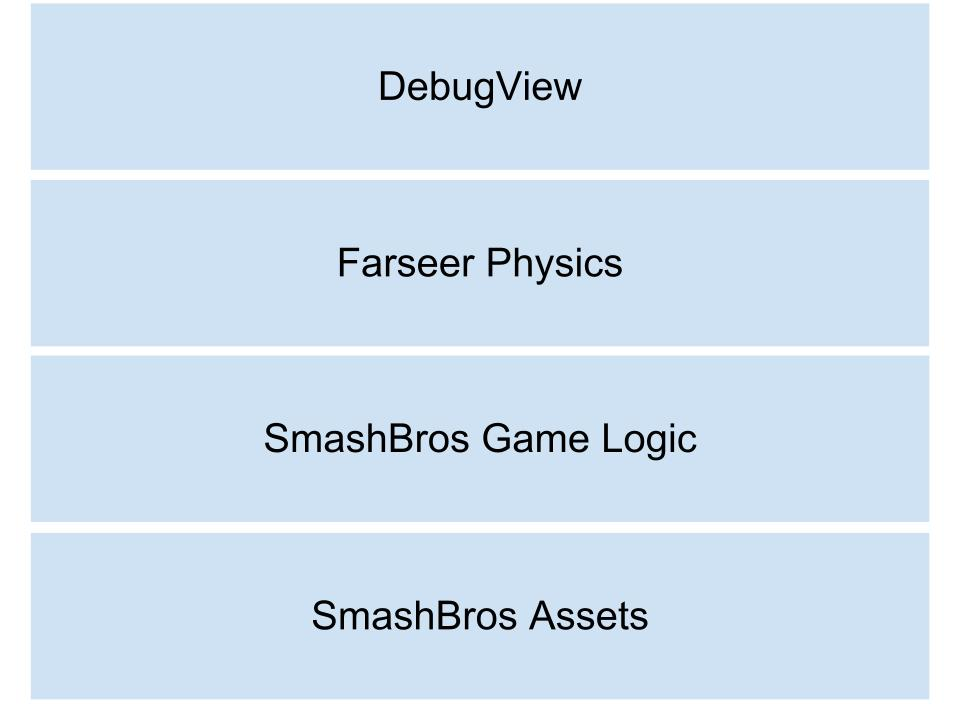
\includegraphics[scale=0.45]{dev.jpg}

\section{State machine}
This is a diagram of our game as a state machine, it covers all the general scenes.
\includegraphics[scale=0.45]{State.jpg}

\section{Consistency among views}
The views are coherent with each other. The logical view excludes the libraries(DebugView and Farseer Physics) and game assets as well as the basic system functions, as they are irrelevant to this view. Scenario view excludes the views of the MVC as those has no game functionality other than viewing. The state machine shows the scenes of the game.

\chapter{Summary}
\section{Architectural Rationale}
We chose MVC as is nicely splits up the game in different categories, it makes both the deveolopment and code review easier as the classes are categorized by functionality. SOA was chosen to increase the modifiability of the game so that it could easily be expanded at a later time by making the classes independant on each other, this knits nicely with observer pattern as it is basically the same thing, only event driven. State machine was selected to nicely split ut the different game states (character selection, options, map selection and game).

\section{Issues}
We found that our architectural patterns worked nicely together, although it was difficult keeping the programming consistent as SOA and OP are very simlar. \\
Had issues keeping the functionality of classes within either models, views or controllers due to time issues.

\chapter{References}
This is the references we used to complete this document 
\section{Books}
\begin{itemize}
\item "Software Architecture in Practice, Second Edition", Len Bass, Paul Clements, Rick Kazman, Addision-Wesley, 2003, ISBN 0-321-15495-9
\item "Game Architecture and Design - A New Edition", Andrew Rollings and Dave Morris
\end{itemize}

\section{Webpages}
\begin{itemize}
\item http://en.wikipedia.org/wiki/SOA
\item http://en.wikipedia.org/wiki/Model–view–controller
\item http://en.wikipedia.org/wiki/Observer\_pattern
\end{itemize}



\chapter{Changes}
29.04.2012\\
Updated based on feedback
\paragraph{}
30.04.2012\\
Added more content to complete the document.

\end{document}